\documentclass{book}
%\reversemarginpar
\usepackage[pass,showframe=true]{geometry}
\newgeometry{top=.5cm,left=4cm,right=2cm,headheight=1cm,headsep=0.5cm,marginpar=3.6cm,
marginparsep=10pt}

\usepackage{lipsum,pgf,caption}
\usepackage[strict]{changepage}
\def\aspectratio{\pgfmathparse{\paperheight/\paperwidth} \pgfmathresult}
\newpage
\newlength\innermargin


\def\printgeometryvalues{\leavevmode
paperwidth \the\paperwidth\\
paperheight \the\paperheight\\
theheadheight \the\headheight\\
theheadsep \the\headsep\\
thetopmargin \the\topmargin\\
theoddsidemargin \the\oddsidemargin\\
theevensidemargin\the\evensidemargin\\
thetextheight\the\textheight\\
themarginparsep \the\marginparsep\\
themarginparwidth \the\marginparwidth\\
themarginpush \the\marginparpush\\
thevoffset \the\voffset
thefootskip \the\footskip\\
aspect ratio \aspectratio\\
topskip \the\topskip\par}

\def\alignedge{%
  \checkoddpage%
  \parindent0pt%
   \ifoddpage \global\setlength\innermargin{\oddsidemargin}
          \else \global\setlength\innermargin{\evensidemargin}
      \fi%
   \if@twoside\setlength\innermargin{\dimexpr(\evensidemargin-\marginparsep)}\else\let\innermargin\oddsidemargin\fi 
 }
\alignedge
\parindent0pt

%\pagecolor{brown}
%\color{white}
\begin{document}
\pagestyle{plain}
\fboxsep0pt\fboxrule0pt
%\checkoddpage

\vspace*{\dimexpr(1in+\headheight+\headsep+\topmargin+\topskip)*(-1)}
\hspace*{\dimexpr(-1in-\innermargin)}%
\fbox{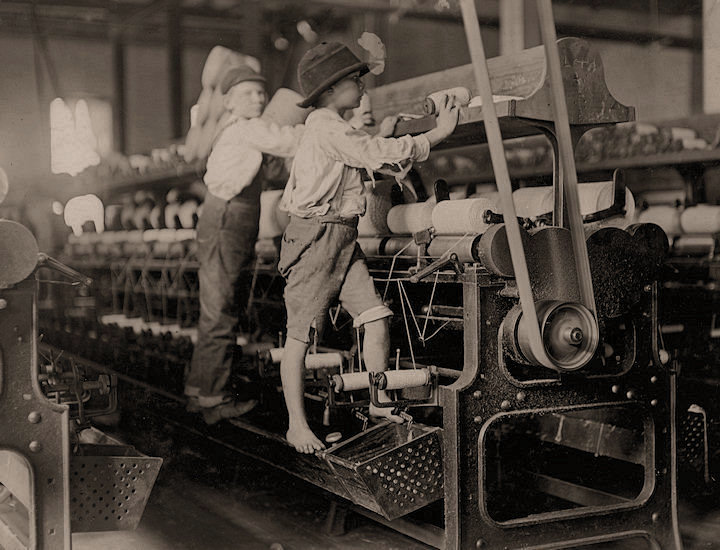
\includegraphics[width=\paperwidth]{./chapters/hine01}}\par
\medskip
\printgeometryvalues


%\checkoddpage
\clearpage
\alignedge
\vspace*{\dimexpr(1in+\headheight+\headsep+\topmargin+\topskip)*(-1)}%
\hspace*{\dimexpr(-1in-\innermargin)}%
\fbox{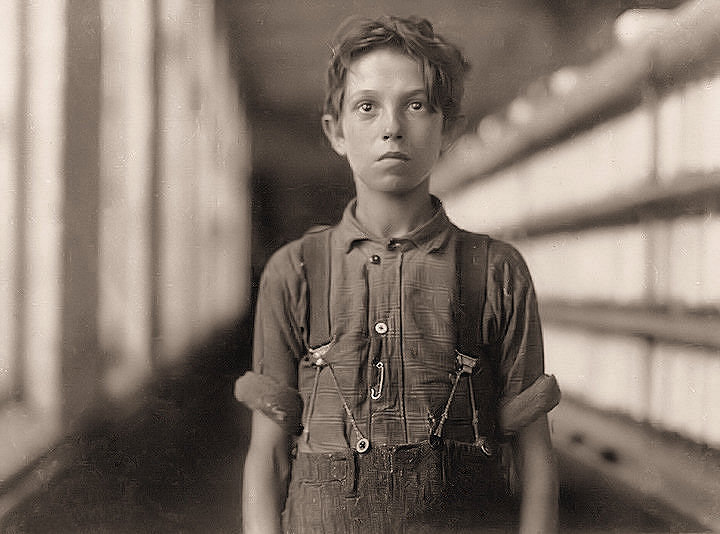
\includegraphics[width=\paperwidth]{./chapters/hine02}}\par
\medskip

\printgeometryvalues
\lipsum


%\checkoddpage
\clearpage
\alignedge
\vspace*{\dimexpr(1in+\headheight+\headsep+\topmargin+\topskip)*(-1)}%
\hspace*{\dimexpr(-1in-\innermargin)}%
\fbox{\includegraphics[width=\paperwidth]{./chapters/hine05}}\par
\medskip
\printgeometryvalues\marginpar{testing}
\lipsum\marginpar{testing}
\lipsum[1-20]
\end{document}